% Options for packages loaded elsewhere
\PassOptionsToPackage{unicode}{hyperref}
\PassOptionsToPackage{hyphens}{url}
\PassOptionsToPackage{dvipsnames,svgnames,x11names}{xcolor}
%
\documentclass[
  letterpaper,
  DIV=11,
  numbers=noendperiod]{scrartcl}

\usepackage{amsmath,amssymb}
\usepackage{lmodern}
\usepackage{iftex}
\ifPDFTeX
  \usepackage[T1]{fontenc}
  \usepackage[utf8]{inputenc}
  \usepackage{textcomp} % provide euro and other symbols
\else % if luatex or xetex
  \usepackage{unicode-math}
  \defaultfontfeatures{Scale=MatchLowercase}
  \defaultfontfeatures[\rmfamily]{Ligatures=TeX,Scale=1}
\fi
% Use upquote if available, for straight quotes in verbatim environments
\IfFileExists{upquote.sty}{\usepackage{upquote}}{}
\IfFileExists{microtype.sty}{% use microtype if available
  \usepackage[]{microtype}
  \UseMicrotypeSet[protrusion]{basicmath} % disable protrusion for tt fonts
}{}
\makeatletter
\@ifundefined{KOMAClassName}{% if non-KOMA class
  \IfFileExists{parskip.sty}{%
    \usepackage{parskip}
  }{% else
    \setlength{\parindent}{0pt}
    \setlength{\parskip}{6pt plus 2pt minus 1pt}}
}{% if KOMA class
  \KOMAoptions{parskip=half}}
\makeatother
\usepackage{xcolor}
\setlength{\emergencystretch}{3em} % prevent overfull lines
\setcounter{secnumdepth}{-\maxdimen} % remove section numbering
% Make \paragraph and \subparagraph free-standing
\ifx\paragraph\undefined\else
  \let\oldparagraph\paragraph
  \renewcommand{\paragraph}[1]{\oldparagraph{#1}\mbox{}}
\fi
\ifx\subparagraph\undefined\else
  \let\oldsubparagraph\subparagraph
  \renewcommand{\subparagraph}[1]{\oldsubparagraph{#1}\mbox{}}
\fi

\usepackage{color}
\usepackage{fancyvrb}
\newcommand{\VerbBar}{|}
\newcommand{\VERB}{\Verb[commandchars=\\\{\}]}
\DefineVerbatimEnvironment{Highlighting}{Verbatim}{commandchars=\\\{\}}
% Add ',fontsize=\small' for more characters per line
\usepackage{framed}
\definecolor{shadecolor}{RGB}{241,243,245}
\newenvironment{Shaded}{\begin{snugshade}}{\end{snugshade}}
\newcommand{\AlertTok}[1]{\textcolor[rgb]{0.68,0.00,0.00}{#1}}
\newcommand{\AnnotationTok}[1]{\textcolor[rgb]{0.37,0.37,0.37}{#1}}
\newcommand{\AttributeTok}[1]{\textcolor[rgb]{0.40,0.45,0.13}{#1}}
\newcommand{\BaseNTok}[1]{\textcolor[rgb]{0.68,0.00,0.00}{#1}}
\newcommand{\BuiltInTok}[1]{\textcolor[rgb]{0.00,0.23,0.31}{#1}}
\newcommand{\CharTok}[1]{\textcolor[rgb]{0.13,0.47,0.30}{#1}}
\newcommand{\CommentTok}[1]{\textcolor[rgb]{0.37,0.37,0.37}{#1}}
\newcommand{\CommentVarTok}[1]{\textcolor[rgb]{0.37,0.37,0.37}{\textit{#1}}}
\newcommand{\ConstantTok}[1]{\textcolor[rgb]{0.56,0.35,0.01}{#1}}
\newcommand{\ControlFlowTok}[1]{\textcolor[rgb]{0.00,0.23,0.31}{#1}}
\newcommand{\DataTypeTok}[1]{\textcolor[rgb]{0.68,0.00,0.00}{#1}}
\newcommand{\DecValTok}[1]{\textcolor[rgb]{0.68,0.00,0.00}{#1}}
\newcommand{\DocumentationTok}[1]{\textcolor[rgb]{0.37,0.37,0.37}{\textit{#1}}}
\newcommand{\ErrorTok}[1]{\textcolor[rgb]{0.68,0.00,0.00}{#1}}
\newcommand{\ExtensionTok}[1]{\textcolor[rgb]{0.00,0.23,0.31}{#1}}
\newcommand{\FloatTok}[1]{\textcolor[rgb]{0.68,0.00,0.00}{#1}}
\newcommand{\FunctionTok}[1]{\textcolor[rgb]{0.28,0.35,0.67}{#1}}
\newcommand{\ImportTok}[1]{\textcolor[rgb]{0.00,0.46,0.62}{#1}}
\newcommand{\InformationTok}[1]{\textcolor[rgb]{0.37,0.37,0.37}{#1}}
\newcommand{\KeywordTok}[1]{\textcolor[rgb]{0.00,0.23,0.31}{#1}}
\newcommand{\NormalTok}[1]{\textcolor[rgb]{0.00,0.23,0.31}{#1}}
\newcommand{\OperatorTok}[1]{\textcolor[rgb]{0.37,0.37,0.37}{#1}}
\newcommand{\OtherTok}[1]{\textcolor[rgb]{0.00,0.23,0.31}{#1}}
\newcommand{\PreprocessorTok}[1]{\textcolor[rgb]{0.68,0.00,0.00}{#1}}
\newcommand{\RegionMarkerTok}[1]{\textcolor[rgb]{0.00,0.23,0.31}{#1}}
\newcommand{\SpecialCharTok}[1]{\textcolor[rgb]{0.37,0.37,0.37}{#1}}
\newcommand{\SpecialStringTok}[1]{\textcolor[rgb]{0.13,0.47,0.30}{#1}}
\newcommand{\StringTok}[1]{\textcolor[rgb]{0.13,0.47,0.30}{#1}}
\newcommand{\VariableTok}[1]{\textcolor[rgb]{0.07,0.07,0.07}{#1}}
\newcommand{\VerbatimStringTok}[1]{\textcolor[rgb]{0.13,0.47,0.30}{#1}}
\newcommand{\WarningTok}[1]{\textcolor[rgb]{0.37,0.37,0.37}{\textit{#1}}}

\providecommand{\tightlist}{%
  \setlength{\itemsep}{0pt}\setlength{\parskip}{0pt}}\usepackage{longtable,booktabs,array}
\usepackage{calc} % for calculating minipage widths
% Correct order of tables after \paragraph or \subparagraph
\usepackage{etoolbox}
\makeatletter
\patchcmd\longtable{\par}{\if@noskipsec\mbox{}\fi\par}{}{}
\makeatother
% Allow footnotes in longtable head/foot
\IfFileExists{footnotehyper.sty}{\usepackage{footnotehyper}}{\usepackage{footnote}}
\makesavenoteenv{longtable}
\usepackage{graphicx}
\makeatletter
\def\maxwidth{\ifdim\Gin@nat@width>\linewidth\linewidth\else\Gin@nat@width\fi}
\def\maxheight{\ifdim\Gin@nat@height>\textheight\textheight\else\Gin@nat@height\fi}
\makeatother
% Scale images if necessary, so that they will not overflow the page
% margins by default, and it is still possible to overwrite the defaults
% using explicit options in \includegraphics[width, height, ...]{}
\setkeys{Gin}{width=\maxwidth,height=\maxheight,keepaspectratio}
% Set default figure placement to htbp
\makeatletter
\def\fps@figure{htbp}
\makeatother

\KOMAoption{captions}{tableheading}
\makeatletter
\makeatother
\makeatletter
\makeatother
\makeatletter
\@ifpackageloaded{caption}{}{\usepackage{caption}}
\AtBeginDocument{%
\ifdefined\contentsname
  \renewcommand*\contentsname{Table of contents}
\else
  \newcommand\contentsname{Table of contents}
\fi
\ifdefined\listfigurename
  \renewcommand*\listfigurename{List of Figures}
\else
  \newcommand\listfigurename{List of Figures}
\fi
\ifdefined\listtablename
  \renewcommand*\listtablename{List of Tables}
\else
  \newcommand\listtablename{List of Tables}
\fi
\ifdefined\figurename
  \renewcommand*\figurename{Figure}
\else
  \newcommand\figurename{Figure}
\fi
\ifdefined\tablename
  \renewcommand*\tablename{Table}
\else
  \newcommand\tablename{Table}
\fi
}
\@ifpackageloaded{float}{}{\usepackage{float}}
\floatstyle{ruled}
\@ifundefined{c@chapter}{\newfloat{codelisting}{h}{lop}}{\newfloat{codelisting}{h}{lop}[chapter]}
\floatname{codelisting}{Listing}
\newcommand*\listoflistings{\listof{codelisting}{List of Listings}}
\makeatother
\makeatletter
\@ifpackageloaded{caption}{}{\usepackage{caption}}
\@ifpackageloaded{subcaption}{}{\usepackage{subcaption}}
\makeatother
\makeatletter
\@ifpackageloaded{tcolorbox}{}{\usepackage[many]{tcolorbox}}
\makeatother
\makeatletter
\@ifundefined{shadecolor}{\definecolor{shadecolor}{rgb}{.97, .97, .97}}
\makeatother
\makeatletter
\makeatother
\ifLuaTeX
  \usepackage{selnolig}  % disable illegal ligatures
\fi
\IfFileExists{bookmark.sty}{\usepackage{bookmark}}{\usepackage{hyperref}}
\IfFileExists{xurl.sty}{\usepackage{xurl}}{} % add URL line breaks if available
\urlstyle{same} % disable monospaced font for URLs
\hypersetup{
  pdftitle={Introduction to Deep Neural Networks},
  pdfauthor={A. Sanchez, F. Reverter and E. Vegas},
  colorlinks=true,
  linkcolor={blue},
  filecolor={Maroon},
  citecolor={Blue},
  urlcolor={Blue},
  pdfcreator={LaTeX via pandoc}}

\title{Introduction to Deep Neural Networks}
\author{A. Sanchez, F. Reverter and E. Vegas}
\date{}

\begin{document}
\maketitle
\ifdefined\Shaded\renewenvironment{Shaded}{\begin{tcolorbox}[boxrule=0pt, interior hidden, borderline west={3pt}{0pt}{shadecolor}, sharp corners, breakable, enhanced, frame hidden]}{\end{tcolorbox}}\fi

\hypertarget{overview-of-deep-learning}{%
\section{Overview of Deep Learning}\label{overview-of-deep-learning}}

\hypertarget{historical-background-1}{%
\subsection{Historical Background (1)}\label{historical-background-1}}

\begin{itemize}
\item
  Today, in April 2023, our world is convulsed by the explosion of
  Artificial Intelligence.
\item
  It has probably been in the last months (weeks), since ChatGPT has
  arrived, that everybody has an opinion, or a fear on the topic.
\end{itemize}

\begin{figure}

{\centering \includegraphics[width=1\textwidth,height=\textheight]{https://bernardmarr.com/wp-content/uploads/2022/04/The-Dangers-Of-Not-Aligning-Artificial-Intelligence-With-Human-Values.jpg}

}

\end{figure}

\hypertarget{historical-background-2}{%
\subsection{Historical Background (2)}\label{historical-background-2}}

\begin{itemize}
\item
  We don't discuss ethical, technological or sociological aspects, but
  is ``\emph{most of this is about prediction}''.
\item
  Most AI engines rely on powerful prediction systems that use
  statistical learning methods.
\end{itemize}

\hypertarget{deep-learning}{%
\subsection{Deep learning}\label{deep-learning}}

\begin{itemize}
\item
  Deep learning is a successful AI model which has powered many
  application such as \emph{self-driving cars, voice assistants, and
  medical diagnosis systems}.
\item
  Essentially, deep learning extends the basic principles of artificial
  neural networks by

  \begin{itemize}
  \tightlist
  \item
    Adding complex architectures and algorithms and
  \item
    At the same time becoming more automatical
  \end{itemize}
\item
  We won't delve into the history of ANN, but a quick look at it may
  help fully grasp its current capabilities.
\end{itemize}

\hypertarget{the-early-history-of-ai-1}{%
\subsection{The early history of AI
(1)}\label{the-early-history-of-ai-1}}

\begin{figure}

{\centering 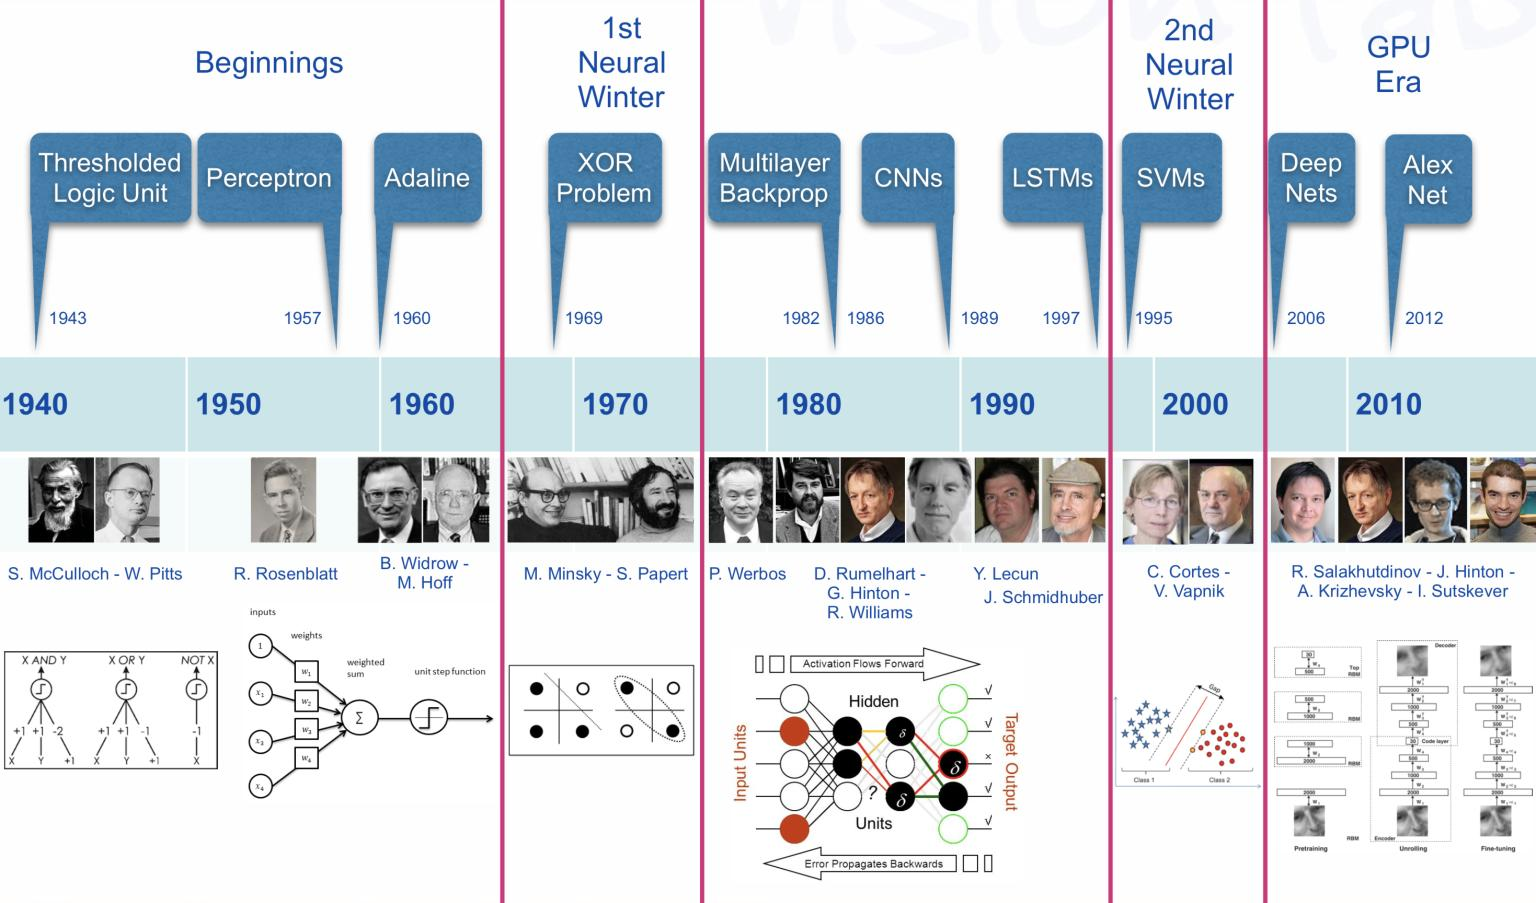
\includegraphics[width=1\textwidth,height=\textheight]{images/AIHistory1.jpg}

}

\caption{A Brief History of AI from 1940s till Today}

\end{figure}

\begin{itemize}
\tightlist
\item
  The origins of AI, and as such of DL can be traced almost one century
  backwards;
\item
  \protect\hypertarget{AIHistory}{\href{https://nerdyelectronics.com/a-quick-history-of-ai-ml-and-dl/}{A
  Quick History of AI, ML and DL}}
\end{itemize}

\hypertarget{milestones-in-the-history-of-dl}{%
\subsection{Milestones in the history of
DL}\label{milestones-in-the-history-of-dl}}

We can see several hints worth to account for:

\begin{itemize}
\item
  The \textbf{Perceptron} and the first \textbf{Artificial Neural
  Network} where the basic building block was introduced.
\item
  The \textbf{Multilayered perceptron} and \textbf{backpropagation}
  where complex architechtures were suggested to improve the
  capabilities.
\item
  \textbf{Deep Neural Networks}, with many hidden layers, and
  auto-tunability capabilities.
\end{itemize}

\hypertarget{from-artificial-neural-networks-to-deep-learning}{%
\subsection{From Artificial Neural Networks to Deep
learning}\label{from-artificial-neural-networks-to-deep-learning}}

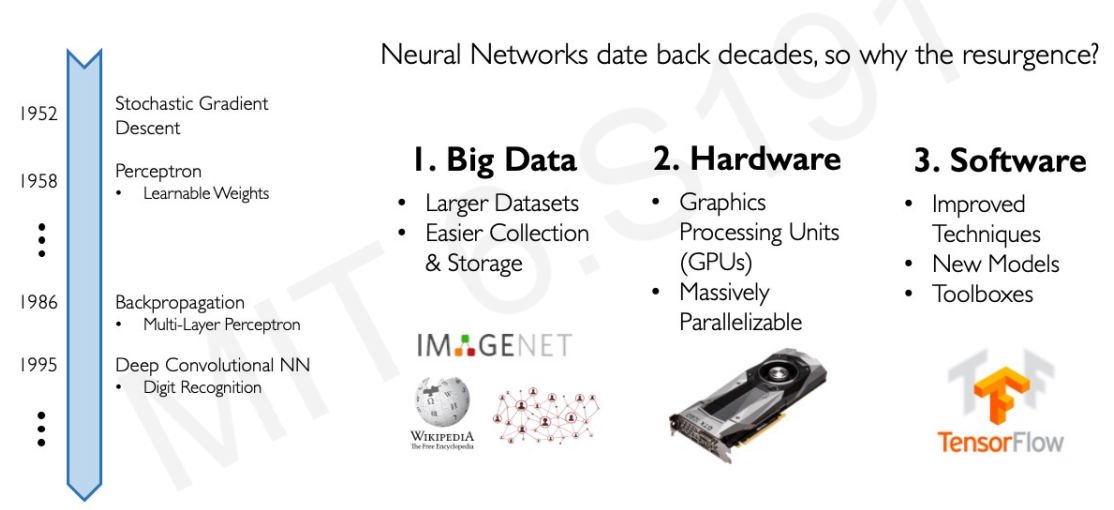
\includegraphics[width=1\textwidth,height=\textheight]{images/WhyDLNow.png}
Source: Alex Amini's `MIT Introduction to Deep Learning' course
(introtodeeplearning.com)

\hypertarget{success-stories}{%
\subsection{Success stories}\label{success-stories}}

Success stories such as

\begin{itemize}
\item
  the development of self-driving cars,
\item
  the use of AI in medical diagnosis, and
\item
  the creation of personalized recommendations in online shopping
\end{itemize}

have also contributed to the widespread adoption of AI.

\hypertarget{ai-ml-dl}{%
\subsection{AI, ML, DL \ldots{}}\label{ai-ml-dl}}

\begin{Shaded}
\begin{Highlighting}[]
\NormalTok{knitr}\SpecialCharTok{::}\FunctionTok{include\_graphics}\NormalTok{(}\StringTok{"images/AI{-}ML{-}DL{-}1.jpg"}\NormalTok{)}
\end{Highlighting}
\end{Shaded}

\begin{figure}[H]

{\centering 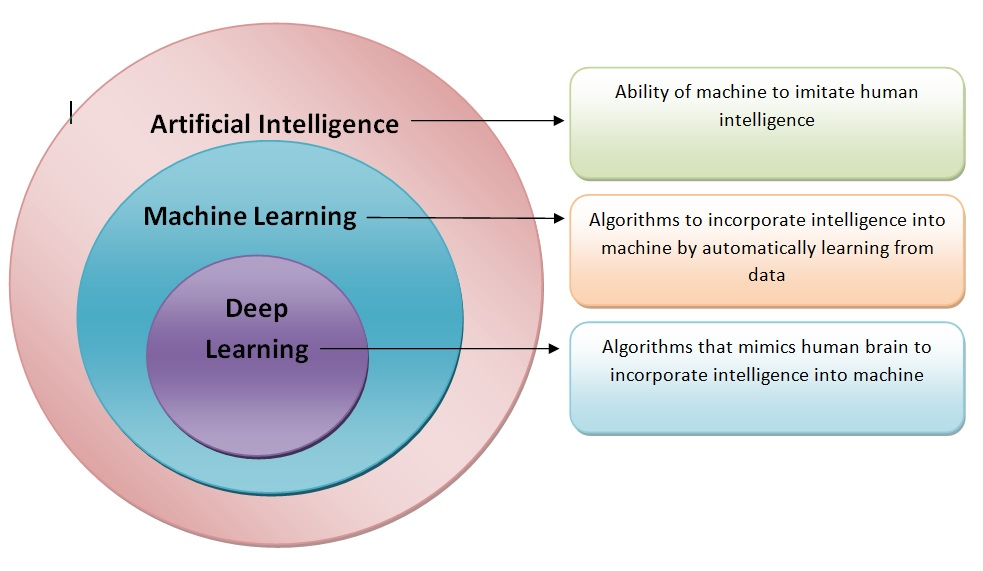
\includegraphics[width=1\textwidth,height=\textheight]{images/AI-ML-DL-1.jpg}

}

\end{figure}

\hypertarget{ai-ml-dl-1}{%
\subsection{AI, ML, DL \ldots{}}\label{ai-ml-dl-1}}

\begin{itemize}
\item
  Artificial intelligence: Ability of a computer to perform tasks
  commonly associated with intelligent beings.
\item
  Machine learning: study of algorithms that learn from examples and
  experience instead of relying on hard-coded rules and make predictions
  on new data
\item
  Deep learning: subfield of ML focusing on learning data
  representations as successive successive layers of increasingly
  meaningful representations.
\end{itemize}

\hypertarget{machine-vs-deep-learning}{%
\subsection{Machine vs Deep Learning}\label{machine-vs-deep-learning}}

\begin{itemize}
\tightlist
\item
  DNN: feature extraction and classification without (or with much les)
  human intervention.
\item
  DNN improves with data availability, without seemingly reaching
  plateaus.
\end{itemize}

\begin{Shaded}
\begin{Highlighting}[]
\NormalTok{knitr}\SpecialCharTok{::}\FunctionTok{include\_graphics}\NormalTok{(}\StringTok{"images/ML\_vs\_DL{-}2.png"}\NormalTok{)}
\end{Highlighting}
\end{Shaded}

\begin{figure}[H]

{\centering 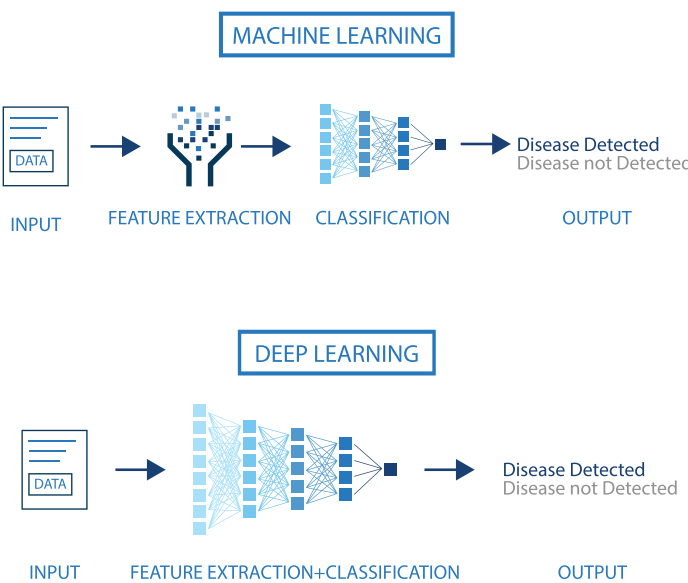
\includegraphics[width=1\textwidth,height=\textheight]{images/ML_vs_DL-2.png}

}

\end{figure}

\hypertarget{size-is-important}{%
\subsection{Size is important!}\label{size-is-important}}

\begin{figure}

{\centering 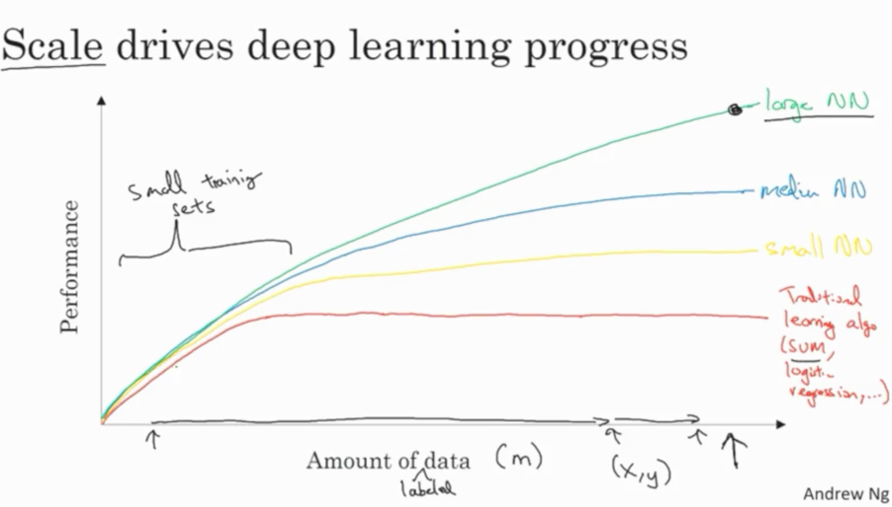
\includegraphics[width=1\textwidth,height=\textheight]{images/PerformanceVsAmountOfData.png}

}

\caption{An illustration of the performance comparison between deep
learning (DL) and other machine learning (ML) algorithms, where DL
modeling from large amounts of data can increase the performance}

\end{figure}

\hypertarget{the-impact-of-deep-learning}{%
\subsection{The impact of Deep
learning}\label{the-impact-of-deep-learning}}

\begin{itemize}
\item
  Near-human-level image classification
\item
  Near-human-level speech transcription
\item
  Near-human-level handwriting transcription
\item
  Dramatically improved machine translation
\item
  Dramatically improved text-to-speech conversion
\item
  Digital assistants such as Google Assistant and Amazon Alexa
\item
  Near-human-level autonomous driving
\item
  Improved ad targeting, as used by Google, Baidu, or Bing
\item
  Improved search results on the web
\item
  Ability to answer natural language questions
\item
  Superhuman Go playing
\end{itemize}

\hypertarget{not-all-that-glitters-is-gold}{%
\subsection{Not all that glitters is gold
\ldots{}}\label{not-all-that-glitters-is-gold}}

\begin{itemize}
\item
  According to F. Chollet, the developer of Keras,

  \begin{itemize}
  \tightlist
  \item
    ``\emph{we shouldn't believe the short-term hype, but should believe
    in the long-term vision}.
  \item
    \emph{It may take a while for AI to be deployed to its true
    potential---a potential the full extent of which no one has yet
    dared to dream}
  \item
    \emph{but AI is coming, and it will transform our world in a
    fantastic way}''.
  \end{itemize}
\end{itemize}

\hypertarget{artificial-neural-networks}{%
\section{Artificial Neural Networks}\label{artificial-neural-networks}}

\hypertarget{the-perceptron-the-building-block}{%
\subsection{The perceptron, the building
block}\label{the-perceptron-the-building-block}}

\begin{itemize}
\item
  The perceptron, was introduced in the 50's (one version of the
  perceptron at least), as a mathematical model that might emulate a
  neuron.
\item
  The idea is: \emph{how can we produce a model that given some inputs,
  and an appropriate set of examples, learn to produce the desired
  output}?
\end{itemize}

\hypertarget{mc-culloughs-neurone}{%
\subsection{Mc Cullough's neurone}\label{mc-culloughs-neurone}}

\begin{itemize}
\tightlist
\item
  The first computational model of a neuron was proposed by Warren
  MuCulloch (neuroscientist) and Walter Pitts (logician) in 1943.
\end{itemize}

\begin{figure}

{\centering 

\href{https://towardsdatascience.com/mcculloch-pitts-model-5fdf65ac5dd1}{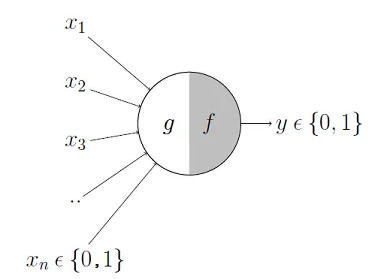
\includegraphics[width=0.93\textwidth,height=\textheight]{images/MacCulloghPitts-Neuron.png}}

}

\end{figure}

\hypertarget{mc-culloughs-neurone-1}{%
\subsection{Mc Cullough's neurone}\label{mc-culloughs-neurone-1}}

\begin{itemize}
\tightlist
\item
  It may be divided into 2 parts.

  \begin{itemize}
  \tightlist
  \item
    The first part, \(g\),takes an input (ahem dendrite ahem),
  \item
    It performs an aggregation and
  \item
    based on the aggregated value the second part, \(f\), makes a
    decision.
  \end{itemize}
\end{itemize}

See
\href{https://towardsdatascience.com/mcculloch-pitts-model-5fdf65ac5dd1}{the
source of this picture} for an illustration on how this can be used to
emulate logical operations such as AND, OR or NOT, but not XOR.

\hypertarget{limitations}{%
\subsection{Limitations}\label{limitations}}

This first attempt to emulate neurons succeeded but with limitations:

\begin{itemize}
\item
  What about non-boolean (say, real) inputs?
\item
  What if all inputs are not equal?
\item
  What if we want to assign more importance to some inputs?
\item
  What about functions which are not linearly separable? Say XOR
  function
\end{itemize}

\hypertarget{overcoming-the-limitations}{%
\subsection{Overcoming the
limitations}\label{overcoming-the-limitations}}

\begin{itemize}
\item
  To overcome these limitations Frank Rosenblatt, proposed the classical
  perception model, the \emph{artificial neuron}, in 1958.
\item
  It is more generalized computational model than the McCulloch-Pitts
  neuron where weights and thresholds can be learnt over time.
\item
  Rosenblatt's perceptron is very similar to an M-P neuron but

  \begin{itemize}
  \tightlist
  \item
    It takes a weighted sum of the inputs and
  \item
    It sets the output as one only when the sum is more than an
    arbitrary threshold (\textbf{\emph{theta}}).
  \end{itemize}
\end{itemize}

\hypertarget{rosenblatts-perceptron}{%
\subsection{Rosenblatt's perceptron}\label{rosenblatts-perceptron}}

\begin{figure}

{\centering 

\href{https://towardsdatascience.com/perceptron-the-artificial-neuron-4d8c70d5cc8d}{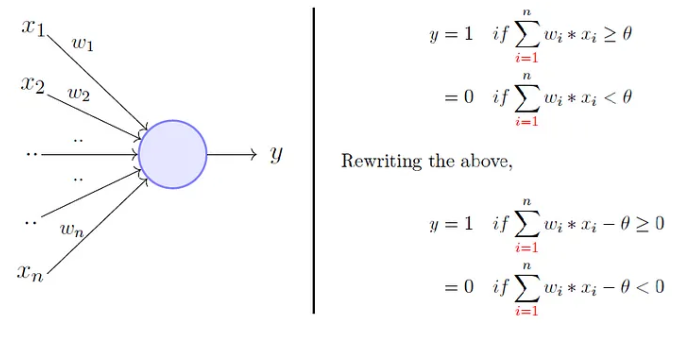
\includegraphics[width=1\textwidth,height=\textheight]{images/RosenblattPerceptron1.png}}

}

\end{figure}

\hypertarget{rosenblatts-perceptron-1}{%
\subsection{Rosenblatt's perceptron
(1)}\label{rosenblatts-perceptron-1}}

\begin{itemize}
\tightlist
\item
  Instead of hand coding the thresholding parameter \(\theta\),
\item
  It is added as one of the inputs, with the weight \(w_0=-\theta\).
\end{itemize}

\begin{figure}

{\centering 

\href{https://towardsdatascience.com/perceptron-the-artificial-neuron-4d8c70d5cc8d}{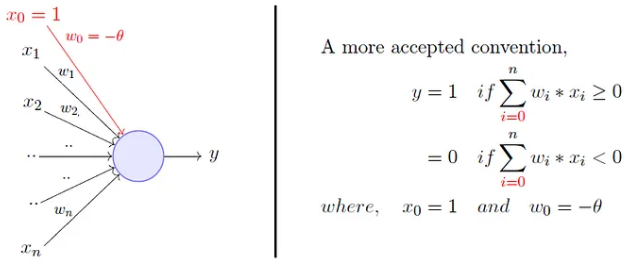
\includegraphics[width=1\textwidth,height=\textheight]{images/RosenblattPerceptron2.png}}

}

\end{figure}

\hypertarget{comparison-between-the-two}{%
\subsection{Comparison between the
two}\label{comparison-between-the-two}}

\begin{figure}

{\centering 

\href{https://towardsdatascience.com/perceptron-the-artificial-neuron-4d8c70d5cc8d}{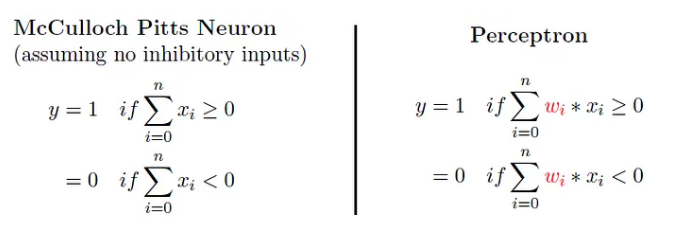
\includegraphics[width=1\textwidth,height=\textheight]{images/McCullaughVSRosenblattPerceptron.png}}

}

\end{figure}

\hypertarget{comparison-between-the-two-1}{%
\subsection{Comparison between the
two}\label{comparison-between-the-two-1}}

\begin{itemize}
\item
  This is an improvement because

  \begin{itemize}
  \tightlist
  \item
    both, weights and threshold, can be learned and
  \item
    the inputs can be real values
  \end{itemize}
\item
  But there is still a drawback in that a single perceptron can only be
  used to implement linearly separable functions.
\item
  Artificial Neural Networks improve on this by introducing
  \emph{Activation Functions}
\end{itemize}

\hypertarget{activation-in-biological-neurons}{%
\subsection{Activation in biological
neurons}\label{activation-in-biological-neurons}}

\begin{itemize}
\tightlist
\item
  Biological neurons are specialized cells in the CNS that transmit
  electrical and chemical signals to communicate with each other.
\item
  The neuron's activation is based on the release of neurotransmitters,
  chemical substances that transmit signals between nerve cells.

  \begin{itemize}
  \tightlist
  \item
    When the signal reaching the neuron exceeds a certain threshold, the
    neuron releases neurotransmitters to continue the communication
    process.
  \end{itemize}
\end{itemize}

\hypertarget{activation-functions-in-an}{%
\subsection{Activation functions in
AN}\label{activation-functions-in-an}}

\begin{itemize}
\tightlist
\item
  Analogously, \emph{activation functions} in AN are functions to decide
  if the AN it is activated or not.
\item
  In AN, the activation function is a mathematical function applied to
  the neuron's input to produce an output.

  \begin{itemize}
  \tightlist
  \item
    In practice it extends to complicated functions that can learn
    complex patterns in the data.
  \item
    Activation functions can incorporate non-linearity, improving over
    linear classifiers.
  \end{itemize}
\end{itemize}

\hypertarget{activation-function}{%
\subsection{Activation function}\label{activation-function}}

\begin{Shaded}
\begin{Highlighting}[]
\NormalTok{knitr}\SpecialCharTok{::}\FunctionTok{include\_graphics}\NormalTok{(}\StringTok{"images/ActivationFunction0.png"}\NormalTok{)}
\end{Highlighting}
\end{Shaded}

\begin{figure}[H]

{\centering 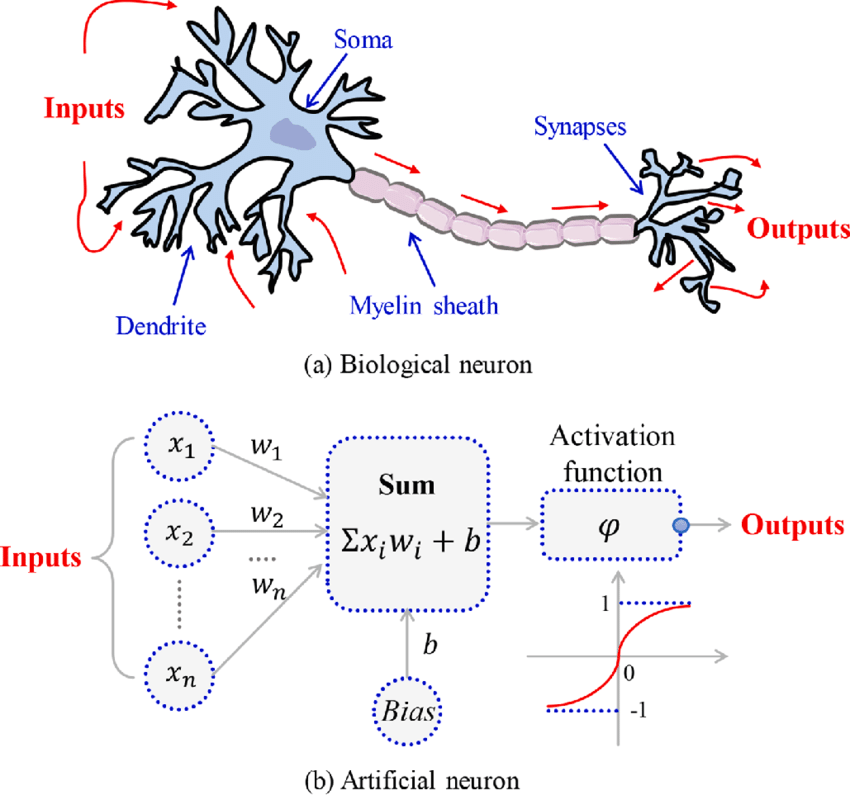
\includegraphics[width=1\textwidth,height=\textheight]{images/ActivationFunction0.png}

}

\end{figure}

\hypertarget{artificial-neuron}{%
\subsection{Artificial Neuron}\label{artificial-neuron}}

With all these ideas in mind we can now define an Artificial Neuron as a
\emph{computational unit} that :

\begin{itemize}
\item
  takes as input \(x=(x_0,x_1,x_2,x_3)\) (\(x_0\) = +1, called bias),
\item
  outputs
  \(h_{\theta}(x) = f(\theta^\intercal x) = f(\sum_i \theta_ix_i)\),
\item
  where \(f:\mathbb{R}\mapsto \mathbb{R}\) is called the
  \textbf{activation function}.
\end{itemize}

\hypertarget{activation-functions}{%
\subsection{Activation functions}\label{activation-functions}}

\begin{itemize}
\item
  Goal of activation function is to provide the neuron with \emph{the
  capability of producing the required outputs}.
\item
  Flexible enough to produce

  \begin{itemize}
  \tightlist
  \item
    Either linear or non-linear transformations.
  \item
    Output in the desired range ({[}0,1{]}, \{-1,1\},
    \(\mathbb{R}^+\)\ldots)
  \end{itemize}
\item
  Usually chosen from a (small) set of possibilities.

  \begin{itemize}
  \tightlist
  \item
    Sigmoid function:
  \item
    Hyperbolic tangent, or \texttt{tanh}, function
  \item
    ReLU
  \end{itemize}
\end{itemize}

\hypertarget{the-sigmoid-function}{%
\subsection{The sigmoid function}\label{the-sigmoid-function}}

\[
f(z)=\frac{1}{1+e^{-z}}
\]

\begin{itemize}
\item
  Output real values \(\in (0,1)\).
\item
  Natural interpretations as \emph{probabilit} of an event
\item
  \emph{vanishing gradient} problem
\item
  Its derivative is: \(f'(z)=f(z)(1-f(z))\).
\end{itemize}

\begin{Shaded}
\begin{Highlighting}[]
\NormalTok{knitr}\SpecialCharTok{::}\FunctionTok{include\_graphics}\NormalTok{(}\StringTok{"images/SigmoidFunction.png"}\NormalTok{)}
\end{Highlighting}
\end{Shaded}

\begin{figure}[H]

{\centering 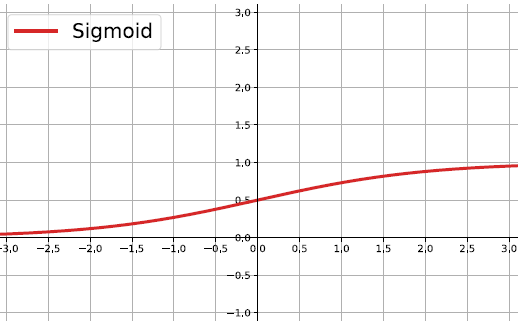
\includegraphics[width=1\textwidth,height=\textheight]{images/SigmoidFunction.png}

}

\end{figure}

\hypertarget{the-hyperbolic-tangent}{%
\subsection{the hyperbolic tangent}\label{the-hyperbolic-tangent}}

Also called \texttt{tanh}, function:

\[
f(z)=\frac{e^{z}-e^{-z}}{e^{z}+e^{-z}}
\]

\begin{itemize}
\item
  outputs are zero-centered and bounded in −1,1
\item
  scaled and shifted Sigmoid
\item
  stronger gradient but still has vanishing gradient problem
\item
  Its derivative is \(f'(z)=1-(f(z))^2\).
\end{itemize}

\begin{Shaded}
\begin{Highlighting}[]
\NormalTok{knitr}\SpecialCharTok{::}\FunctionTok{include\_graphics}\NormalTok{(}\StringTok{"images/TanhFunction.png"}\NormalTok{)}
\end{Highlighting}
\end{Shaded}

\begin{figure}[H]

{\centering 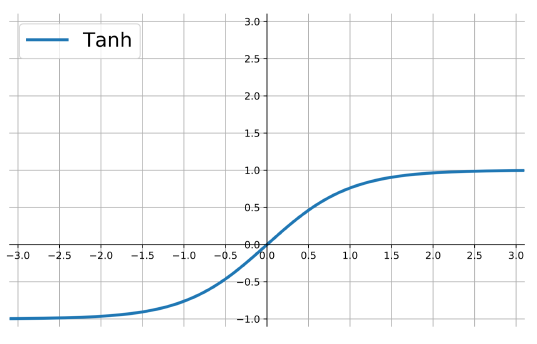
\includegraphics[width=1\textwidth,height=\textheight]{images/TanhFunction.png}

}

\end{figure}

\hypertarget{the-relu}{%
\subsection{The ReLU}\label{the-relu}}

\begin{itemize}
\item
  \emph{rectified linear unit}: \(f(z)=\max\{0,z\}\).
\item
  Close to a linear: \emph{piecewise linear} function with two linear
  pieces.
\item
  Outputs are in \%(0,\infty)\$ , thus not bounded
\item
  Half rectified: activation threshold at 0
\item
  No vanishing gradient problem
\end{itemize}

\begin{Shaded}
\begin{Highlighting}[]
\NormalTok{knitr}\SpecialCharTok{::}\FunctionTok{include\_graphics}\NormalTok{(}\StringTok{"images/ReLUFunction.png"}\NormalTok{)}
\end{Highlighting}
\end{Shaded}

\begin{figure}[H]

{\centering 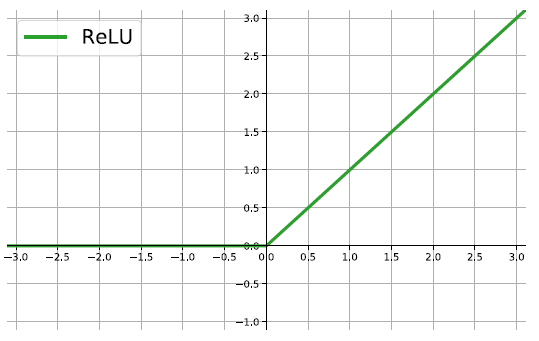
\includegraphics[width=1\textwidth,height=\textheight]{images/ReLUFunction.png}

}

\end{figure}

\hypertarget{more-activation-functions}{%
\subsection{More activation functions}\label{more-activation-functions}}

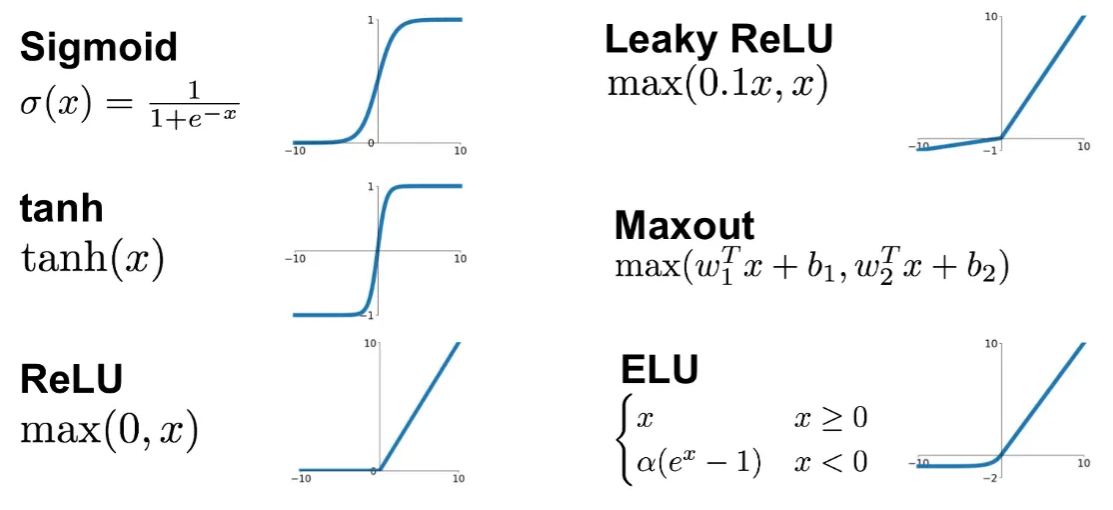
\includegraphics[width=1\textwidth,height=\textheight]{images/ActivationFunctions.png}.

\hypertarget{putting-it-all-together}{%
\subsection{Putting it all together}\label{putting-it-all-together}}

\begin{Shaded}
\begin{Highlighting}[]
\NormalTok{knitr}\SpecialCharTok{::}\FunctionTok{include\_graphics}\NormalTok{(}\StringTok{"images/ArtificialNeuron.png"}\NormalTok{)}
\end{Highlighting}
\end{Shaded}

\begin{figure}[H]

{\centering 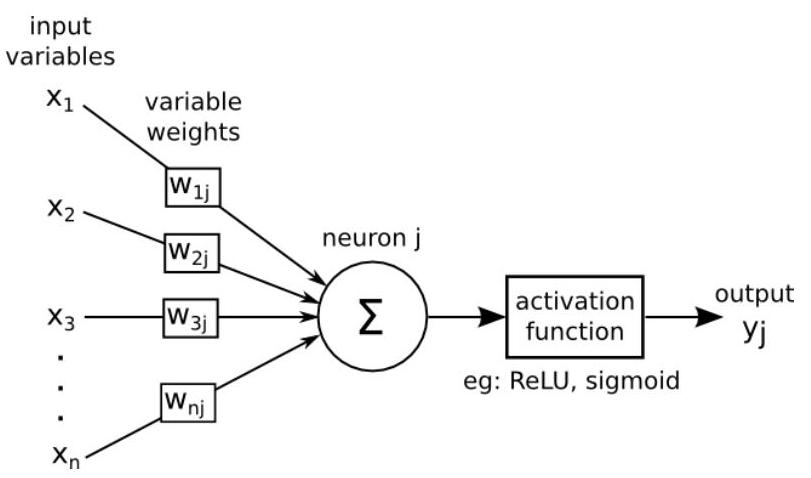
\includegraphics[width=1\textwidth,height=\textheight]{images/ArtificialNeuron.png}

}

\end{figure}

\(\Sigma=\left\langle w_{j}, x\right\rangle+ b_{j}\)

\hypertarget{multilayer-perceptrons}{%
\subsection{Multilayer perceptrons}\label{multilayer-perceptrons}}

\begin{itemize}
\tightlist
\item
  A Multilayer Perceptron or Artificial Neural Network (ANN) is a
  computational model that mimics the structure and function of the
  human brain.
\item
  It is composed of interconnected nodes, called neurons, that are
  organized into layers.
\item
  Neurons in each layer are connected to neurons in the next layer,
  forming a directed graph-like structure.
\item
  The first layer (input layer) receives input data.
\item
  Last layer produces the final prediction
\item
  Intermediate (hidden) layers perform intermediate calculatuions.
\end{itemize}

\hypertarget{an-artificial-neural-network}{%
\subsection{An Artificial Neural
network}\label{an-artificial-neural-network}}

\begin{Shaded}
\begin{Highlighting}[]
\NormalTok{knitr}\SpecialCharTok{::}\FunctionTok{include\_graphics}\NormalTok{(}\StringTok{"images/MultiLayer1.png"}\NormalTok{)}
\end{Highlighting}
\end{Shaded}

\begin{figure}[H]

{\centering 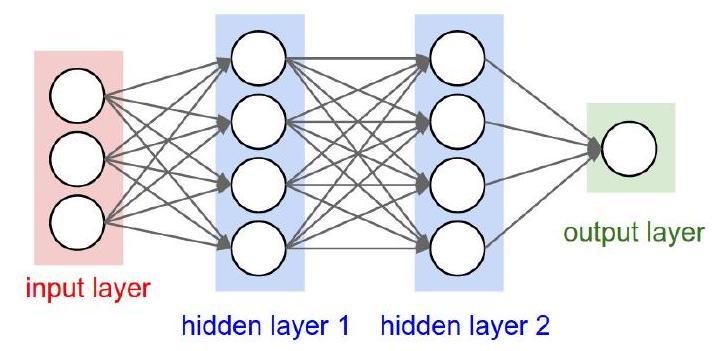
\includegraphics[width=1\textwidth,height=\textheight]{images/MultiLayer1.png}

}

\end{figure}

\hypertarget{the-architechture-of-ann}{%
\subsection{The architechture of ANN}\label{the-architechture-of-ann}}

\begin{itemize}
\item
  Multilayers perceptrons have a basic architecture since each unit (or
  neuron) of a layer is linked to all the units of the next layer but
  has no link with the neurons of the same layer.
\item
  The parameters of the architecture are:

  \begin{itemize}
  \tightlist
  \item
    the number of hidden layers and
  \item
    the number of neurons in each layer.
  \item
    The activation functions
  \end{itemize}
\end{itemize}

\hypertarget{activation-functions-for-ann-1}{%
\subsection{Activation functions for ANN
(1)}\label{activation-functions-for-ann-1}}

\begin{itemize}
\tightlist
\item
  For the output layer, the activation function is generally different
  from the one used on the hidden layers.

  \begin{itemize}
  \tightlist
  \item
    For \textbf{regression}, we apply no activation function on the
    output layer.
  \item
    For \textbf{binary} classification, where output is a prediction of
    \(\mathbb{P}(Y=1 /X) \in [0,1]\)

    \begin{itemize}
    \tightlist
    \item
      The \emph{sigmoid} activation function is used.
    \end{itemize}
  \item
    For \textbf{multi-class classification}, where ther is one neuron
    per class giving a prediction of \(\mathbb{P}(Y=i / X)\).

    \begin{itemize}
    \tightlist
    \item
      The \emph{softmax} activation function is common
    \end{itemize}
  \end{itemize}
\end{itemize}

\hypertarget{the-softmax-activation-function}{%
\subsection{The softmax activation
function}\label{the-softmax-activation-function}}

\[
\operatorname{softmax}(z)_{i}=\frac{\exp \left(z_{i}\right)}{\sum_{j} \exp \left(z_{j}\right)}
\]

\hypertarget{an-example}{%
\section{An example}\label{an-example}}

\hypertarget{a-predictive-ann}{%
\subsection{A predictive ANN}\label{a-predictive-ann}}

We use the \texttt{neuralnet} package to build a simple neural network
to predict if a type of stock pays dividends or not.

\begin{Shaded}
\begin{Highlighting}[]
\ControlFlowTok{if}\NormalTok{ (}\SpecialCharTok{!}\FunctionTok{require}\NormalTok{(neuralnet)) }
  \FunctionTok{install.packages}\NormalTok{(}\StringTok{"neuralnet"}\NormalTok{, }\AttributeTok{dep=}\ConstantTok{TRUE}\NormalTok{)}
\end{Highlighting}
\end{Shaded}

\begin{verbatim}
Loading required package: neuralnet
\end{verbatim}

\begin{verbatim}
Warning: package 'neuralnet' was built under R version 4.2.3
\end{verbatim}

\hypertarget{data-for-the-example}{%
\subsection{Data for the example}\label{data-for-the-example}}

And use the \texttt{dividendinfo.csv} dataset from
\url{https://github.com/MGCodesandStats/datasets}

\begin{Shaded}
\begin{Highlighting}[]
\NormalTok{mydata }\OtherTok{\textless{}{-}} \FunctionTok{read.csv}\NormalTok{(}\StringTok{"https://raw.githubusercontent.com/MGCodesandStats/datasets/master/dividendinfo.csv"}\NormalTok{)}
\FunctionTok{str}\NormalTok{(mydata)}
\end{Highlighting}
\end{Shaded}

\begin{verbatim}
'data.frame':   200 obs. of  6 variables:
 $ dividend       : int  0 1 1 0 1 1 1 0 1 1 ...
 $ fcfps          : num  2.75 4.96 2.78 0.43 2.94 3.9 1.09 2.32 2.5 4.46 ...
 $ earnings_growth: num  -19.25 0.83 1.09 12.97 2.44 ...
 $ de             : num  1.11 1.09 0.19 1.7 1.83 0.46 2.32 3.34 3.15 3.33 ...
 $ mcap           : int  545 630 562 388 684 621 656 351 658 330 ...
 $ current_ratio  : num  0.924 1.469 1.976 1.942 2.487 ...
\end{verbatim}

\hypertarget{data-preprocessing}{%
\subsection{Data preprocessing}\label{data-preprocessing}}

\begin{Shaded}
\begin{Highlighting}[]
\NormalTok{normalize }\OtherTok{\textless{}{-}} \ControlFlowTok{function}\NormalTok{(x) \{}
  \FunctionTok{return}\NormalTok{ ((x }\SpecialCharTok{{-}} \FunctionTok{min}\NormalTok{(x)) }\SpecialCharTok{/}\NormalTok{ (}\FunctionTok{max}\NormalTok{(x) }\SpecialCharTok{{-}} \FunctionTok{min}\NormalTok{(x)))}
\NormalTok{\}}
\NormalTok{normData }\OtherTok{\textless{}{-}} \FunctionTok{as.data.frame}\NormalTok{(}\FunctionTok{lapply}\NormalTok{(mydata, normalize))}
\end{Highlighting}
\end{Shaded}

\hypertarget{test-and-training-sets}{%
\subsection{Test and training sets}\label{test-and-training-sets}}

Finally we break our data in a test and a training set:

\begin{Shaded}
\begin{Highlighting}[]
\NormalTok{perc2Train }\OtherTok{\textless{}{-}} \DecValTok{2}\SpecialCharTok{/}\DecValTok{3}
\NormalTok{ssize }\OtherTok{\textless{}{-}} \FunctionTok{nrow}\NormalTok{(normData)}
\FunctionTok{set.seed}\NormalTok{(}\DecValTok{12345}\NormalTok{)}
\NormalTok{data\_rows }\OtherTok{\textless{}{-}} \FunctionTok{floor}\NormalTok{(perc2Train }\SpecialCharTok{*}\NormalTok{ssize)}
\NormalTok{train\_indices }\OtherTok{\textless{}{-}} \FunctionTok{sample}\NormalTok{(}\FunctionTok{c}\NormalTok{(}\DecValTok{1}\SpecialCharTok{:}\NormalTok{ssize), data\_rows)}
\NormalTok{trainset }\OtherTok{\textless{}{-}}\NormalTok{ normData[train\_indices,]}
\NormalTok{testset }\OtherTok{\textless{}{-}}\NormalTok{ normData[}\SpecialCharTok{{-}}\NormalTok{train\_indices,]}
\end{Highlighting}
\end{Shaded}

\hypertarget{training-a-neural-network}{%
\subsection{Training a neural network}\label{training-a-neural-network}}

We train a simple NN with two hidden layers, with 4 and 2 neurons
respectively.

\begin{Shaded}
\begin{Highlighting}[]
\CommentTok{\#Neural Network}
\FunctionTok{library}\NormalTok{(neuralnet)}
\NormalTok{nn }\OtherTok{\textless{}{-}} \FunctionTok{neuralnet}\NormalTok{(dividend }\SpecialCharTok{\textasciitilde{}}\NormalTok{ fcfps }\SpecialCharTok{+}\NormalTok{ earnings\_growth }\SpecialCharTok{+}\NormalTok{ de }\SpecialCharTok{+}\NormalTok{ mcap }\SpecialCharTok{+}\NormalTok{ current\_ratio, }
                \AttributeTok{data=}\NormalTok{trainset, }
                \AttributeTok{hidden=}\FunctionTok{c}\NormalTok{(}\DecValTok{2}\NormalTok{,}\DecValTok{1}\NormalTok{), }
                \AttributeTok{linear.output=}\ConstantTok{FALSE}\NormalTok{, }
                \AttributeTok{threshold=}\FloatTok{0.01}\NormalTok{)}
\end{Highlighting}
\end{Shaded}

\hypertarget{network-plot}{%
\subsection{Network plot}\label{network-plot}}

The output of the procedure is a neural network with estimated weights

\begin{Shaded}
\begin{Highlighting}[]
\FunctionTok{plot}\NormalTok{(nn, }\AttributeTok{rep =} \StringTok{"best"}\NormalTok{)}
\end{Highlighting}
\end{Shaded}

\begin{figure}[H]

{\centering 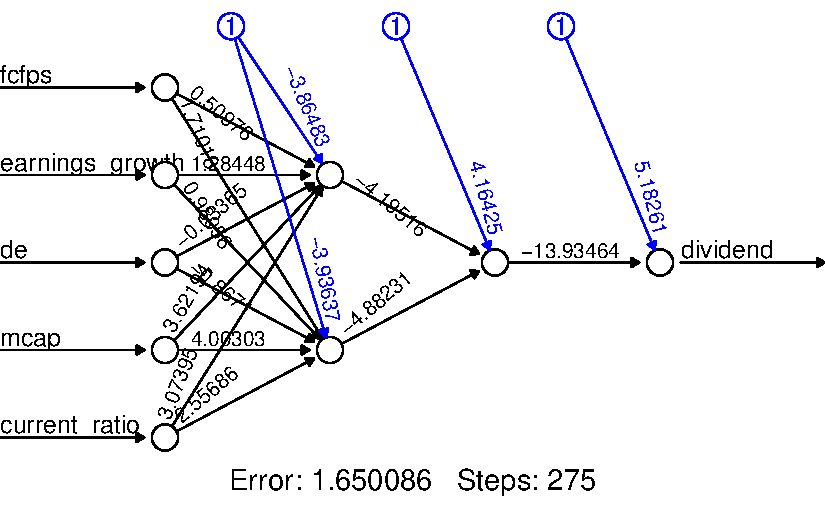
\includegraphics{2-Intro2DeepLearning_files/figure-pdf/unnamed-chunk-14-1.pdf}

}

\end{figure}

\hypertarget{predictions}{%
\subsection{Predictions}\label{predictions}}

\begin{Shaded}
\begin{Highlighting}[]
\NormalTok{temp\_test }\OtherTok{\textless{}{-}} \FunctionTok{subset}\NormalTok{(testset, }\AttributeTok{select =}
                      \FunctionTok{c}\NormalTok{(}\StringTok{"fcfps"}\NormalTok{,}\StringTok{"earnings\_growth"}\NormalTok{, }
                        \StringTok{"de"}\NormalTok{, }\StringTok{"mcap"}\NormalTok{, }\StringTok{"current\_ratio"}\NormalTok{))}
\NormalTok{nn.results }\OtherTok{\textless{}{-}} \FunctionTok{compute}\NormalTok{(nn, temp\_test)}
\NormalTok{results }\OtherTok{\textless{}{-}} \FunctionTok{data.frame}\NormalTok{(}\AttributeTok{actual =} 
\NormalTok{                  testset}\SpecialCharTok{$}\NormalTok{dividend, }
                  \AttributeTok{prediction =}\NormalTok{ nn.results}\SpecialCharTok{$}\NormalTok{net.result)}
\FunctionTok{head}\NormalTok{(results)}
\end{Highlighting}
\end{Shaded}

\begin{verbatim}
   actual   prediction
9       1 0.9919213885
19      1 0.9769206123
22      0 0.0002187144
26      0 0.6093330933
27      1 0.7454164893
29      1 0.9515431416
\end{verbatim}

\hypertarget{model-evaluation}{%
\subsection{Model evaluation}\label{model-evaluation}}

\begin{Shaded}
\begin{Highlighting}[]
\NormalTok{roundedresults}\OtherTok{\textless{}{-}}\FunctionTok{sapply}\NormalTok{(results,round,}\AttributeTok{digits=}\DecValTok{0}\NormalTok{)}
\NormalTok{roundedresultsdf}\OtherTok{=}\FunctionTok{data.frame}\NormalTok{(roundedresults)}
\FunctionTok{attach}\NormalTok{(roundedresultsdf)}
\FunctionTok{table}\NormalTok{(actual,prediction)}
\end{Highlighting}
\end{Shaded}

\begin{verbatim}
      prediction
actual  0  1
     0 33  3
     1  4 27
\end{verbatim}

\hypertarget{some-mathematics-behind-ann}{%
\section{Some mathematics behind
ANN}\label{some-mathematics-behind-ann}}

\hypertarget{mathematical-formulation}{%
\subsection{Mathematical formulation}\label{mathematical-formulation}}

\begin{itemize}
\item
  An ANN is a predictive model whose functioning and properties can be
  mathematically characterized.
\item
  In practice this means describing

  \begin{itemize}
  \tightlist
  \item
    The ANN as a (non linear) function.
  \item
    The (optimization) process for estimating the weights.
  \end{itemize}
\end{itemize}

\hypertarget{estimating-the-weights}{%
\subsection{Estimating the weights}\label{estimating-the-weights}}

\begin{itemize}
\tightlist
\item
  In order to use the ANN for prediction, weights need to be estimated.
\item
  This is done by minimizing an appropriate loss function which requires

  \begin{itemize}
  \tightlist
  \item
    An appropriate procedure: \emph{gradient based optimization}
  \item
    A method for computing the required derivatives:
    \emph{back-propagation}.
  \end{itemize}
\end{itemize}

\hypertarget{a-guiding-example}{%
\subsection{A guiding example}\label{a-guiding-example}}

\begin{itemize}
\tightlist
\item
  Input layer with 3 input units (plus bias unit),
\item
  1 hidden layer with 3 hidden units,
\item
  Output layer with 1 output unit.
\end{itemize}

\begin{Shaded}
\begin{Highlighting}[]
\NormalTok{knitr}\SpecialCharTok{::}\FunctionTok{include\_graphics}\NormalTok{(}\StringTok{"images/nn.jpg"}\NormalTok{)}
\end{Highlighting}
\end{Shaded}

\begin{figure}[H]

{\centering 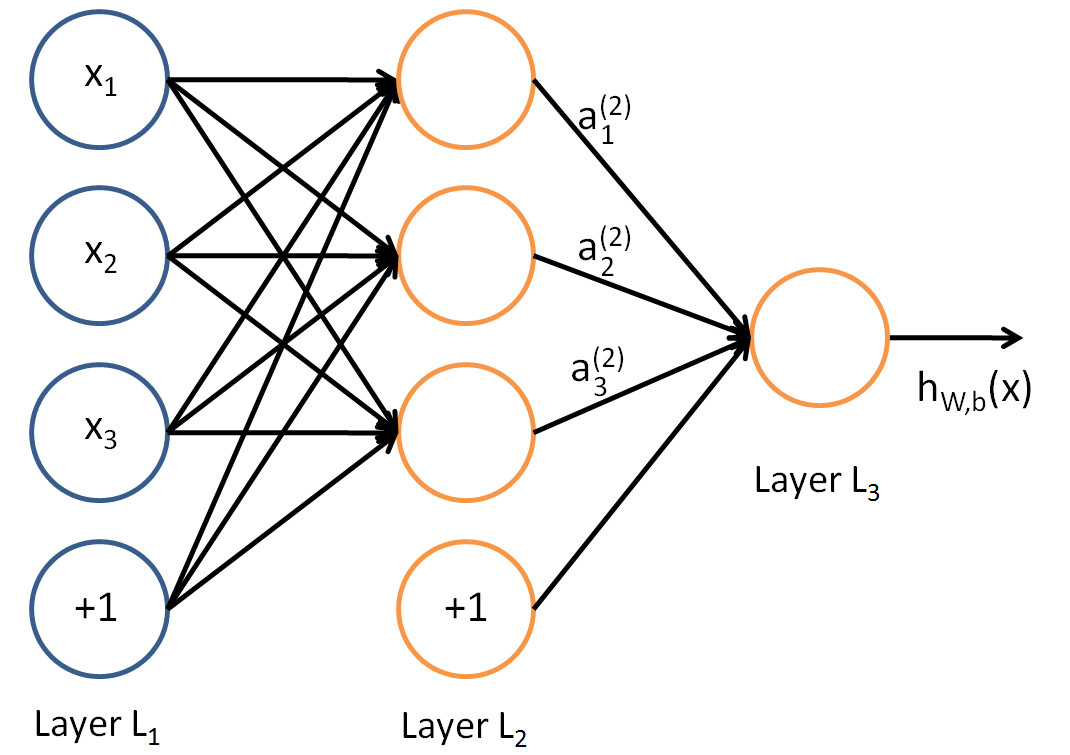
\includegraphics[width=1\textwidth,height=\textheight]{images/nn.jpg}

}

\end{figure}

\hypertarget{a-logistic-regression-ann}{%
\subsection{A logistic regression ANN}\label{a-logistic-regression-ann}}

This ANN can be seen as a logistic regression model:

\begin{itemize}
\item
  From input layer to layer 2: non-linear transformation
  --\textgreater{} new set of complex features.
\item
  From layer 2 to output layer use a sigmoid activation function to
  produce the following output from the set of \emph{complex features}.
\end{itemize}

\[
\mbox{The output is: }h_{\theta}(x)=\frac{1}{1+e^{-\theta^\intercal x}}
\]

\hypertarget{logistic-regression-1}{%
\subsection{Logistic regression (1)}\label{logistic-regression-1}}

Recall that, the logistic regression model is:

\[
\log\frac{p(Y=1|x)}{1-p(Y=1|x)}=\theta^\intercal x
\]

Isolating \(p(Y=1|x)\) and taking logs in both sides, we have:

\[
\frac{p(Y=1|x)}{1-p(Y=1|x)}=e^{\theta^\intercal x}
\]

\hypertarget{logistic-regression-2}{%
\subsection{Logistic regression (2)}\label{logistic-regression-2}}

\[
p(Y=1|x)=\frac{e^{\theta^\intercal x}}{1+e^{\theta^\intercal x}}=\frac{1}{1+e^{-\theta^\intercal x}}
\]

\begin{itemize}
\item
  That is: \emph{when the activation function of the output node is the
  sigmoid activation function, the output coincides with a logistic
  regression on complex features}
\item
  And, with \(h_{\theta}(x)\), the output of the NN, we are estimating
  \(p(Y=1|x)\).
\end{itemize}

\hypertarget{an-ann-has-weights-parameters}{%
\subsection{\texorpdfstring{An ANN has weights =
\emph{parameters}}{An ANN has weights = parameters}}\label{an-ann-has-weights-parameters}}

\begin{itemize}
\tightlist
\item
  Let \(n_l\) denote the number of layers in our network, thus \(n_l=3\)
  in our example.
\item
  Label layer \(l\) as \(L_l\), so layer \(L_1\) is the input layer, and
  layer \(L_{n_l}=L_3\) the output layer.
\item
  Our neural network has parameters:
  \(\Theta=(\Theta^{(1)},\Theta^{(2)})\), where we will write
  \(\theta^{(l)}_{ij}\) to denote the parameter (or weight) associated
  with the connection between unit \(j\) in layer \(l\), and unit \(i\)
  in layer \(l+1\).
\end{itemize}

\hypertarget{back-to-the-example}{%
\subsection{Back to the example:}\label{back-to-the-example}}

\begin{itemize}
\item
  Thus, in our example, we have:

  \begin{itemize}
  \tightlist
  \item
    \(\Theta^{(1)}\in\mathbb{R}^{3\times 4}\), and
  \item
    \(\Theta^{(2)}\in\mathbb{R}^{1\times 4}\).
  \end{itemize}
\end{itemize}

Note that bias units don't have inputs or connections going into them,
since they always output the value +1.

\hypertarget{the-ann-is-defined-by-its-weights}{%
\subsection{The ANN is defined by its
weights}\label{the-ann-is-defined-by-its-weights}}

\begin{itemize}
\item
  We also let \(s_l\) denote the number of nodes in layer \(l\) (not
  counting the bias unit).
\item
  Now, write \(a^{(l)}_i\) to denote the activation (meaning output
  value) of unit \(i\) in layer \(l\).

  \begin{itemize}
  \tightlist
  \item
    For \(l=1\), we also use \(a^{(1)}_i=x_i\) to denote the \(i\)-th
    input.
  \end{itemize}
\item
  Given a fixed setting of the parameters \(\Theta\), our neural network
  defines a model \(h_{\Theta}(x)\) that outputs a real number.
\end{itemize}

\hypertarget{combining-everything-to-compute}{%
\subsection{Combining everything to
compute}\label{combining-everything-to-compute}}

\begin{itemize}
\item
  We can now see \emph{how these weights are used to produce the
  output}: \begin{eqnarray}
  a_1^{(2)}&=&f(\theta_{10}^{(1)}+\theta_{11}^{(1)}x_1+\theta_{12}^{(1)}x_2+\theta_{13}^{(1)}x_3)\\
  a_2^{(2)}&=&f(\theta_{20}^{(1)}+\theta_{21}^{(1)}x_1+\theta_{22}^{(1)}x_2+\theta_{23}^{(1)}x_3)\\
  a_3^{(2)}&=&f(\theta_{30}^{(1)}+\theta_{31}^{(1)}x_1+\theta_{32}^{(1)}x_2+\theta_{33}^{(1)}x_3)\\
  h_{\Theta}(x)&=&a_1^{(3)}=f(\theta_{10}^{(2)}+\theta_{11}^{(2)}a_1^{(2)}+\theta_{12}^{(2)}a_2^{(2)}+\theta_{13}^{(2)}a_3^{(2)})
  \end{eqnarray}
\item
  Now, letting \(z_i^{(l)}\) denote the total weighted sum of inputs to
  unit \(i\) in layer \(l\), including the bias term
  \[z_i^{(2)}=\theta_{i0}^{(1)}+\theta_{i1}^{(1)}x_1+\theta_{i2}^{(1)}x_2+\theta_{i3}^{(1)}x_3,
  \] the output becomes: \(a_i^{(l)}=f(z_i^{(l)})\).
\end{itemize}

\hypertarget{compacting-notation}{%
\subsection{Compacting notation}\label{compacting-notation}}

\begin{itemize}
\item
  Note that this easily lends itself to a more compact notation.
\item
  Extending the activation function \(f(\cdot)\) to apply to vectors in
  an elementwise fashion: \[
  f([z_1,z_2,z_3]) = [f(z_1), f(z_2),f(z_3)],
  \]
\end{itemize}

then we can write the previous equations more compactly as:

\begin{eqnarray}
z^{(2)}&=&\Theta^{(1)}x\nonumber\\
a^{(2)}&=&f(z^{(2)})\nonumber\\
z^{(3)}&=&\Theta^{(2)}a^{(2)}\nonumber\\
h_{\Theta}(x)&=&a^{(3)}=f(z^{(3)})\nonumber
\end{eqnarray}

\hypertarget{compacting-notation-ii}{%
\subsection{Compacting notation (II)}\label{compacting-notation-ii}}

\begin{itemize}
\item
  More generally, recalling that we also use \(a^{(1)}=x\) to also
  denote the values from the input layer,
\item
  then given layer \(l\)'s activations \(a^{(l)}\), we can compute layer
  \(l+1\)'s activations \(a^{(l+1)}\) as:
\end{itemize}

\begin{eqnarray}
z^{(l+1)}&=&\Theta^{(l)}a^{(l)}\\
a^{(l+1)}&=&f(z^{(l+1)})
\end{eqnarray}

\hypertarget{matricial-representation-i}{%
\subsection{Matricial representation
(I)}\label{matricial-representation-i}}

\[
z^{(l+1)}=
\begin{bmatrix}
z_1^{(l+1)}\\
z_2^{(l+1)}\\
\vdots\\
z_{s_{l+1}}^{(l)}
\end{bmatrix}=
\begin{bmatrix}
\theta_{10}^{(l)}& \theta_{11}^{(l)}&\theta_{12}^{(l)}&...&\theta_{1s_{l}}^{(l)}&\\
\theta_{20}^{(l)}& \theta_{21}^{(l)}&\theta_{22}^{(l)}&...&\theta_{2s_{l}}^{(l)}&\\
\vdots & \vdots& \vdots & \vdots & \vdots\\
\theta_{s_{l+1}0}^{(l)}& \theta_{s_{l+1}1}^{(l)}&\theta_{s_{l+1}2}^{(l)}&...&\theta_{s_{l+1}s_{l}}^{(l)}&\\
\end{bmatrix}
\cdot\begin{bmatrix}
1\\
a_1^{(l)}\\
a_2^{(l)}\\
\vdots\\
a_{s_l}^{(l)}
\end{bmatrix}
\]

\hypertarget{matricial-representation-ii}{%
\subsection{Matricial representation
(II)}\label{matricial-representation-ii}}

The activation is then:

\[
a^{(l+1)}=
\begin{bmatrix}
a_1^{(l+1)}\\
a_2^{(l+1)}\\
\vdots\\
a_{s_{l+1}}^{(l)}
\end{bmatrix}=f(z^{(l+1)})=\begin{bmatrix}
f(z_1^{(l+1)})\\
f(z_2^{(l+1)})\\
\vdots\\
f(z_{s_{l+1}}^{(l)})
\end{bmatrix}
\]

\hypertarget{references-and-resources}{%
\section{References and Resources}\label{references-and-resources}}



\end{document}
